\documentclass{article}

%\title{Effects of User Interface in Communication Delays in Interplanetary Analog Missions}
\title{Bachelor Arbeit}
\author{Christian Gommeringer}
% \authorpronound{his}
% \prevdega{Your Previous Degree \#1}
% \prevdegb{Your Previous Degree \#2}
% \gradmonth{August}
% \gradyear{2024}
% \department{Your Department}
% \cchair{Your committee chair}
% \cmembera{Your committee member \#1}
% \cmemberb{Your committee member \#2}
% \cmemberc{Your committee member \#3}
% \cmemberd{Your committee member \#4}
% \graddean{Name of Grad Dean}

% \abstract{Your abstract goes here. You can also use an input command with a filename.}
% \acknowledgements{Your acknowledgements go here. You can also use an input command with a filename.}
% \dedication{Your dedication goes here.}
\usepackage{amsmath}
\usepackage{amsfonts}
% \usepackage{unicode-math}
\usepackage{amssymb}
\usepackage{braket}
\usepackage{mathtools}
\usepackage[a4paper, margin=2cm]{geometry}
\usepackage{bbold}
\usepackage{graphicx}
\usepackage[toc,page]{appendix}
\usepackage{wrapfig}
\usepackage{hyperref}
\usepackage{floatrow}
\usepackage{subcaption}
\usepackage[backend=biber]{biblatex} %Imports biblatex package
\addbibresource{source.bib}
% \setmathfont{Asana Math}
% \makeglossaries
% \loadglsentries{glossary}

% Right align bibliography to get rid of under full warnings.
% There are two options for this. Preference is to keep bibliography justified. 
%\apptocmd{\thebibliography}{\raggedright}{}{}
% \apptocmd{\sloppy}{\hbadness 10000\relax}{}{}
% \overfullrule=5pt

\begin{document}
\newcommand{\half}{\frac{1}{2}}
\newcommand{\Tr}{\operatorname{Tr}}
\newcommand{\Trs}[1]{\Tr_S\left\{#1\right\}}
\newcommand{\Trb}[1]{\Tr_B\left\{#1\right\}}
% \newcommand{\dt}[1]{\frac{\text{d} #1}{\text{d}t}}
\newcommand{\dt}{\frac{\text{d}}{\text{d}t}}
\newcommand{\tk}{\tilde{\kappa}}
\newcommand{\tw}{\tilde{\omega}}
\newcommand{\dkw}{\left(\frac{\text{d}}{\text{d}{y}}\,\frac{\Omega^2}{K}\right)}
\newcommand{\kw}{\frac{\Omega^2}{K}}
\newcommand{\ty}{{y}}
\newcommand{\diff}{\text{d}}
\maketitle


\section{The model}
In this project I will examine a System of N 2-level atoms or spins, described in a collision model framework\cite{ciccarello_cm,cm_source2}. The system will be under the influence of several interaction types due to coupling to external baths. These effects are captured by the collision model Hamiltonian 
\begin{align*}
    H &= \frac{\delta}{2}\,J_z+ \omega\,J_x+\alpha\,(J_+a + J_-a^\dagger)+ \beta\,J_z\,(b^\dagger+b)+\xi\,\sum_{i=1}^N\,(\sigma_i^-c_i^\dagger+\sigma_i^+c_i)\\
    \text{with}\quad H_S&=\frac{\delta}{2}\,J_z+ \omega\,J_x\\
    V_a&=\alpha\,(J_+a- + J_-a^\dagger)\\
    V_b&=\beta\,J_z\,(b^\dagger+b)\\
    V_c&=\xi\,\sum_{i=1}^N\,(\sigma_i^-c_i^\dagger+\sigma_i^+c_i)\\
    J_k &=\half\,\sum_{j=1}^N\sigma_j^k\quad k\in\{x,y,z\}\\
    J_\pm&=\half\,\sum_{j=1}^N\sigma_j^\pm\\
    \alpha&=\sqrt{\frac{\kappa}{\Delta tN}}\,;\quad \beta=\sqrt{\frac{\gamma}{\Delta t}}\,;\quad \xi=\sqrt{\frac{\Gamma}{4\Delta t}}
\end{align*}
The operators acting on the system are the pauli spin matrices $\sigma^{x,y,z}$. I will go through the terms, where I will label them and explain their derivation. $\delta$ labels the detuning of a laser driving coupled with the parameter $\omega$. The responsible field is treated classically, which is possible if the field is strong enough, so that the behavior of the atoms has no influence on the state of this light field. The term can be derived by starting with the light atom interaction in the dipole approximation.
\begin{align*}
    H = \omega_0\,\ket{e}\bra{e}+ \hat{d}\,\cos(\omega_Lt)\quad,
\end{align*} 
where $\hat{d}$ is the dipole operator multiplied with the external field amplitude
\begin{align*}
    \hat{d}&=\hat{\bf{r}}\,\bf{E_0}\\
    &=2\omega\, \sigma^x
\end{align*}
in the bases of the atomic ground and exited state $\ket{g}$, $\ket{e}$ with $2\omega\vcentcolon=\braket{e|\hat{\bf{r}}\,\bf{E_0}|g}$, what is assumed to be real. The elementary charge shall be contained in $\bf{E_0}$. The diagonal elements vanish because of the parity properties of the states. After transforming the state of the system via the gauge transformation with the unitary $U=\exp(i\omega t)\,\ket{e}\bra{e}+\ket{g}\bra{g}$ the Hamiltonian transforms to 
\begin{align*}
    H\rightarrow \,&UHU^\dagger+i\,(\frac{\diff}{\diff t}\,U)\,U^\dagger\\
    =\,&\omega_0\,\ket{e}\bra{e}-\omega_L\,\ket{e}\bra{e} + 2\omega\,\cos(\omega_L t)\,\{e^{i\omega_L t} \ket{e}\bra{g}+e^{-i\omega_L t}\ket{g}\bra{e}\}\\
    =\,&(\omega_0-\omega_L)\,\ket{e}\bra{e}+\omega\,\sigma_x
\end{align*}
Between the second to third step the counter rotating exponentials have been neglected. By resetting the zero energy point to the middle of the atomic states and defining $\delta=\omega_0-\omega_L$ the Hamiltonian can be written as
\begin{align*}
    H = \frac{\delta}{2}\,\sigma^z+ \omega\,\sigma^x
\end{align*}
The Jaynes-Cummings term can be derived in a similar manner with a quantum field. 
\begin{align*}
    H= \frac{\omega_0}{2}\,\sigma^z+\int_{0}^\infty\diff\omega\,\omega\,a^\dagger_\omega a_\omega+ \hat{\boldsymbol{d}}\,\int_{0}^\infty\diff\omega\,\tilde{\alpha}(\omega)\,\boldsymbol{E_0}\,(a_\omega+a^\dagger_\omega)
\end{align*}
where the dipole approximation has already been performed. By assuming that only a small number of modes actually contribute to the interaction, one can without consequences extend the integral to $-\infty$. I will also assume that within the relevant frequency interval the coupling strength $\tilde{\alpha}$ is constant, making it possible to write the Hamiltonian as
\begin{align*}
    H= \frac{\omega_0}{2}\,\sigma^z+\int_{-\infty}^\infty\diff\omega\,\omega\,a^\dagger_\omega a_\omega+ \alpha\,\int_{-\infty}^\infty\diff\omega\,\sigma^x\,(a_\omega+a^\dagger_\omega)
\end{align*}
By going to the interaction picture with respect to the bosonic bath and neglecting counter rotating terms, we get to the equation
\begin{align*}
    H= \frac{\omega_0}{2}\,\sigma^z+ \alpha\,\int_{-\infty}^\infty\diff\omega\,(e^{-i\omega t}\sigma^+a_\omega+e^{i\omega t}\sigma^-a^\dagger_\omega)
\end{align*}
This resembles the Jaynes-Cummings model in the interaction picture. At this point I want to introduce the collision model approach, which will be used for this project. Starting with the definition
\begin{align*}
    a_t\vcentcolon=\int_{-\infty}^{\infty}\diff\omega\,e^{-i\omega t}a_\omega
\end{align*}
lets the Hamiltonian read
\begin{align*}
    H= \frac{\omega_0}{2}\,\sigma^z+ \alpha\,(\sigma^+a_t+\sigma^-a^\dagger_t)
\end{align*}
The unitary propagation can be decomposed into $N$ consecutive propagations of duration $\Delta t$
\begin{align*}
    U(t,t_0)&=\mathcal{T}\left(  \exp(-i\int_{t_0}^t\diff t'\,H(t'))  \right)=U_{N}\cdots U_1\\
    \text{with}\quad U_n&=\mathcal{T}\left( \exp(-i\int_{t_0+(n-1)\,\Delta t}^{t_0+n\,\Delta t}\diff t'\,H(t'))  \right)
\end{align*}
As can be shown\cite{ciccarello_cm} the propagation can be approximated up to the second order in $\Delta t$ via
\begin{align*}
    U_n \approx 1-i\int_{t_0+(n-1)\,\Delta t}^{t_0+n\,\Delta t}\diff t \,H(t) - \half\,\left(\int_{t_0+(n-1)\,\Delta t}^{t_0+n\,\Delta t}\diff t \,H(t)\right)^2
\end{align*}
After introducing
\begin{align*}
    a_n\vcentcolon&=\frac{1}{\sqrt{\Delta t}}\int_{t_0+(n-1)\,\Delta t}^{t_0+n\,\Delta t}\diff t\,a_t
\end{align*}
and redefining $\alpha\rightarrow\alpha/\sqrt{\Delta t}$ this can be written as
\begin{align*}
    U_n &\approx 1-i\,H_n \,\Delta t-\half\,H_n^2\,\Delta t^2\\
    \text{with}\quad H_n&=\alpha\,(\sigma_+a_n+\sigma_-a^\dagger_n)
\end{align*}
The evolution of the system factorizes into consecutive interactions described by the Hamiltonian $H_n$. Those interactions can be interpreted as $N$ independent bath segments, called in the following ancillas, interacting separately with the system, when the following property holds. At each such interaction the state of the bath is completely uncorrelated  to and not influenced by what has happened during the previous interactions - or at least to a sufficient degree. In this case the main criteria for a description through the collision model are met, which are \cite{ciccarello_cm}:
\begin{itemize}
    \item ancillas do not interact with each other 
    \item ancillas are initially uncorrelated 
    \item each ancilla collides with S only once 
\end{itemize}. 
The assumption of independent consecutive interactions leans on the assumption of a correlation time of the bath, which is much smaller than the one of the system. Note, that $[a_n,a^\dagger_{n'}]=\delta_{n,n'}$ holds, which strengthens the notion of independent modes.\\\\%, and therefore the modes of different $n$ do not depend on each other, which is important for being able to describe the system via a collision model with collisions with ancillas $n$.
in our case the ancillas of the collective Jaynes-Cummings interaction $V_a$ are all prepared in the vacuum state, and thus the interaction describes the spontaneous emission of the atoms.\\\\
The Term $V_b$ resembles a dephasing process, which can be simulated via spin-dependent kick operations\cite{exp_spin_boson}. The last interaction $V_c$ introduces another Jaynes-Cummings term, where each spin is individually coupled to a bosonic bath. Each ancilla will be set in the first exited state. Thus this interaction constitutes a local pumping process.

\section{Derivation of the Lindblad equation}
In order to derive the Lindblad equation from the collision we will continue from the propagation by the single ancilla,
\begin{align*}
    U_n &\approx 1-i\,H_n \,\Delta t-\half\,H_n^2\,\Delta t^2
\end{align*}
and decompose the Hamiltonian in a term that solely effect the System and one that describes the interaction with the baths.
\begin{align*}
    H_n &= H_n^S + V_n\\
    H_n^S&=\frac{\delta}{2}\,J_z+\omega\,J_x\\
    V_n&= \alpha\,(J_+a_n + J_-a_n^\dagger)+ \beta\,J_z\,(b_n^\dagger+b_n)+\xi\,\sum_{i=1}^N\,(\sigma_{i}^-c_{n,i}^\dagger+\sigma_i^+c_{n,i})
\end{align*}
Now the propagation of the density matrix $\chi$ of the composite system ($\rho$) and ancilla ($\eta_n$). As assumed they initially are uncorrelated $\chi_n=\rho_n\otimes\eta_n$, where $\rho_n$ is the density matrix of the system at the beginning of the $n$th $\Delta t$-interval.
\begin{align*}
    \rho_{n+1}\otimes\eta_n((n+1)\,\Delta t)&=U_n\chi_nU_n^\dagger
\end{align*}
Here $\eta_m((n+1)\,\Delta t)$ represents the state of the ancilla at the end of the interaction.
If one no plugs in the approximate form of the propagation $U_n$, one reaches at
\begin{align*}
    \rho_{n+1}\otimes\eta_n((n+1)\,\Delta t)-\rho_n\otimes\eta_n&=-i\,[H_n,\chi_n]\,\Delta t+H_n\,\chi_n\,H_n\,\Delta t^2+\half\,[H_n^2,\chi]_+\,\Delta t^2
\end{align*}
where $[\cdot,\cdot]_+$ is the anticommutation relation. If one now neglects the terms quadratic in $H_n^S$, as is explained in \cite{ciccarello_cm}, the equation of motion becomes
\begin{align*}
    \rho_{n+1}\otimes\eta_n((n+1)\,\Delta t)-\rho_n\otimes\eta_n=\Delta\chi_n\vcentcolon=-i\,[H_n,\chi_n]\,\Delta t+V_n\,\chi_n\,V_n\,\Delta t^2+\half\,[V_n^2,\chi]_+\,\Delta t^2
\end{align*}
Tracing out the baths leads to the Lindblad equation for the density matrix. In the following I will drop the subscript $n$. As the the expectation values of the interaction operators on the bath side vanish in our case, the first term becomes
\begin{align*}
    L_S=-i\,[H_S,\rho]
    \text{for}\quad \frac{\Delta\rho}{\Delta t}=L_S+L_a+L_b+L_c
\end{align*}
I will go through the different contributions. 
\begin{align*}
    L_a &= \alpha^2\,\Trb{V_a\chi V_a-\half\,[V_a^2,\chi]_+}\,\Delta t\\
    &= \frac{\kappa}{N}\,J_-\rho J_+\,\Trb{a\,a^\dagger\eta_a}-\half\,\frac{\kappa}{N}\,[J_+J_-,\rho]_+\,\Trb{[a\,a^\dagger,\eta_a]_+}\\
    &=\frac{\kappa}{N}\,(J_-\rho J_+-\half\,[J_+J_-,\rho]_+)\\
    \text{for}\quad\eta_a&=\ket{\text{vac}}_a\bra{\text{vac}}
\end{align*}
From the start I excluded the vanishing terms $\Trb{(a^\dagger a^\dagger+a\,a+a^\dagger a)\cdot\eta}$. Analogously can be continued for the other parts of $H$.
\begin{align*}
    L_b&= \beta^2\,J_z\rho J_z\, \Trb{b\,b^\dagger\eta_b}\,\Delta t-\beta^2\,\half\,[J_z^2,\rho]_+\,\Trb{[b\,b^\dagger,\eta_b]_+}\,\Delta t\\
    &=\gamma\,J_z\rho J_z-\half\,\gamma\,[J_z^2,\rho]_+\\
    \eta_b&=\ket{\text{vac}}_b\bra{\text{vac}}\\
    L_c&= \xi^2\,\sum_i\sigma_i^-\rho \sigma_i^+\, \Trb{c_i^\dagger c_i\eta^c_i}\,\Delta t-\xi^2\,\half\,\sum_i\,[\sigma_i^-\sigma_i^+,\rho]_+\,\Trb{[c_i^\dagger c_i,\eta^c_i]_+}\,\Delta t\\
    &=\frac{\Gamma}{4}\,\left(\sum_i\sigma_i^-\rho \sigma_i^+-\half\,\sum_i\,[\sigma_i^-\sigma_i^+,\rho]_+\right)\\
    \eta^c_i&=\ket{1}^c_i\bra{1}
\end{align*}
If the interaction with each ancilla gets very short, one can approximately perform the limit $\Delta t\rightarrow0$ and propagate the density matrix of the system continuously through time. The time evolution of the expectation value of an observable $O_S$ can be determined via 
\begin{align*}
    \dt \braket{O_S}=\Trs{O_S\,\dt\rho}&=\Trs{O_S\,(L_S+L_a+L_b+L_c)}\\
    &=\vcentcolon \mathcal{L}_S(O_S)+\mathcal{L}_a(O_S)+\mathcal{L}_b(O_S)+\mathcal{L}_c(O_S)
\end{align*}
With this expression the time evolution of the the spin components can be computed.
\begin{align*}
    \mathcal{L}_S(J_z)&=\omega\,\braket{J_y}\\
    \mathcal{L}_S(J_\pm)&=-i\,\left(\mp\frac{\delta}{2}\, \braket{J_\pm} \pm \omega\, \braket{J_z}\right)
\end{align*}
The interactions with the bath are described in the Lindblad form. The detailed calculations have be shifted to the Appendix \ref{appendix:eqm_derv}. Here I only collect the different contributions to the Lindblad equation for the different interaction types.
\begin{align*}
    \mathcal{L}_a(J_z)=-\frac{\kappa}{N}\,\Trs{J_+ J_- \rho},\quad
    \mathcal{L}_a(J_+)=\frac{\kappa}{N}\,\Trs{J_+ J_z \rho},\quad
    \mathcal{L}_a(J_-)=\frac{\kappa}{N}\,\Trs{J_z J_- \rho}
\end{align*}
\begin{align*}
    \mathcal{L}_b(J_z)=0,\quad
    \mathcal{L}_b(J_\pm)=-\half\,\gamma\,\Trs{J_\pm\rho}
\end{align*}
\begin{align*}
    \mathcal{L}_c(J_z)=\half\,N\,\Gamma-\Gamma\,\braket{J_z},\quad
    \mathcal{L}_c(J_-)=-\frac{\Gamma}{2}\,\sum_{k=1}^N\Trs{\sigma_k^-\rho},\quad
    \mathcal{L}_c(J_+)=-\frac{\Gamma}{2}\,\sum_{k=1}^N\Trs{\sigma_k^+\rho}
\end{align*}
Putting everything together the equations of motion read
\begin{align*}
    \dt \braket{J_+}&=\,i\,\frac{\delta}{2}\,\braket{J_+}-i\,\omega\,\braket{J_z}-\half\,(\gamma+\Gamma)\,\braket{J_+}+\frac{\kappa}{N}\,\braket{J_+ J_z}\\
    \dt \braket{J_-}&=-i\,\frac{\delta}{2}\,\braket{J_-}+i\,\omega\,\braket{J_z}-\half\,(\gamma+\Gamma)\,\braket{J_-}+\frac{\kappa}{N}\,\braket{J_z J_-}\\
    &=-i\,\frac{\delta}{2}\,\braket{J_-}+i\,\omega\,\braket{J_z}-\half\,(\gamma+\Gamma)\,\braket{J_-}+\frac{\kappa}{N}\,\braket{J_- J_z}-\frac{\kappa}{N}\,\braket{J_-}\\
    \dt \braket{J_z}&=\omega\,\braket{J_y} - \frac{\kappa}{N}\,\braket{J_+ J_-}+\half\,N\,\Gamma-\Gamma\,\braket{J_z}
\end{align*}
These can be transformed from the ladder operators back to the spin components.
\begin{align*}
    \dt\,\braket{J_x}=\half\,\left(\dt \braket{J_+}+\dt \braket{J_-}\right)&=-\frac{\delta}{2}\,\braket{J_y}-\half\,(\gamma+\Gamma)\,\braket{J_x}+\frac{\kappa}{N}\,\braket{J_xJ_z}-\frac{\kappa}{2N}\,\braket{J_-}\\
    \dt\,\braket{J_y}=-i\,\half\,\left(\dt \braket{J_+}-\dt \braket{J_-}\right)&=\frac{\delta}{2}\,\braket{J_x}-\omega\,\braket{J_z}-\half\,(\gamma+\Gamma)\,\braket{J_y}+\frac{\kappa}{N}\,\braket{J_yJ_z}-i\,\frac{\kappa}{2N}\,\braket{J_-}\\
    \dt \braket{J_z}&=\omega\,\braket{J_y} - \frac{\kappa}{N}\,\braket{J_x^2+J_y^2} -\frac{\kappa}{N}\,\braket{J_z}+\half\,N\,\Gamma-\Gamma\,\braket{J_z}
\end{align*}
From here I will continue with the mean field approximation $\braket{A\,B}=\braket{A}\,\braket{B}$, and define the mean field expectation values $m_\alpha=\braket{J_\alpha}/N$. I will take the thermodynamic limit $N\rightarrow\infty$, in which the mean field treatment is correct. In this limit terms of the form $\braket{J_\alpha}/N^2\rightarrow0$ vanish. The mean field equations of motion then read
\begin{align*}
    \dt m_x &= -\frac{\delta}{2}\,m_y-\half\,(\gamma+\Gamma)\,m_x+\kappa\,m_x m_z\\
    \dt m_y &= \frac{\delta}{2}\,m_x-\omega\,m_z-\half\,(\gamma+\Gamma)\,m_y+\kappa\,m_y m_z\\
    \dt m_z &= \omega\,m_z - \kappa\,(m_x^2+m_y^2)+\half\Gamma-\Gamma\,m_z
\end{align*}
\section{Evaluating the mean field equations}
As a first step I will examine properties of the total spin
\begin{align*}
    m^2\vcentcolon&=m_x^2+m_y^2+m_z^2\\
    \Rightarrow\quad\dt m^2&=2\,\left( m_x\,\dt m_x +m_y\,\dt m_y +m_z\,\dt m_z \right)\\
    &=-\vec{m}^t\,\left( \begin{array}{ccc}
        \Gamma+\gamma & 0&0  \\
        0& \Gamma+\gamma & 0\\
        0&0&2\,\Gamma
   \end{array}\right)\,\vec{m}+\Gamma\,m_z\\
   &=-\left(  (\Gamma+\gamma)\,(m_x^2+m_y^2)+2\,\Gamma\,m_z^2-\Gamma\,m_z \right)
\end{align*}
From this expression one can already say that laser driving, detuning and spontaneous emission have no direct influence on the total spin modulus. Further can be recognized that in the case, where there is no pumping present, the dephasing term drives the system into a fully mixed state, which follows from the negative definiteness of the derivative of total spin modulus. The proof of this intuitively understandable statement can be found in the Appendix \ref{appendix:msq_calc}. Therefore for interesting things to happen in this model, a pumping process has to be implemented.

\subsection{Zero detuning}
We proceed by solving the set of mean field equations for stationary states, i.e. $\text{d}/\text{d}t\,m_x=\text{d}/\text{d}t\,m_y=\text{d}/\text{d}t\,m_z=0$. The $m_z$-equation can be reformulated as
\begin{align*}
    m_z=\half-\frac{1}{\Gamma}\,\left(\kappa\,(m_x^2+ m_y^2)-\omega\,m_y  \right)
\end{align*}
in the case $\Gamma\neq0$. This makes the problem 2 dimensional.
\begin{align*}
    -\frac{\delta}{2}\,m_y-\half\,(\gamma+\Gamma)\,m_x+\kappa\,m_x\,\left( \half-\frac{1}{\Gamma}\,\left(\kappa\,(m_x^2+ m_y^2)-\omega\,m_y  \right)  \right)&=0\\
    \frac{\delta}{2}\,m_x-\omega\,\left( \half-\frac{1}{\Gamma}\,\left(\kappa\,(m_x^2+ m_y^2)-\omega\,m_y  \right)  \right)&\\-\half\,(\gamma+\Gamma)\,m_y+\kappa\,m_y\,\left( \half-\frac{1}{\Gamma}\,\left(\kappa\,(m_x^2+ m_y^2)-\omega\,m_y  \right)  \right)&=0\\\\
    \text{multiplying with }2\Gamma\text{ yields}\quad\quad\quad\hspace*{6cm}&
    \\\Rightarrow\quad-\Gamma\delta\,m_y-\Gamma\,(\gamma+\Gamma-\kappa)\,m_x-2\,\kappa^2\,m_x\,( m_x^2+ m_y^2)+2\,\kappa\omega\,m_xm_y  &=0\\\\
    \Gamma\delta\,m_x-\omega\Gamma-\Gamma\,(\gamma+\Gamma-\kappa+2\,\omega^2/\Gamma)\,m_y&\\
    -2\,\kappa^2\,m_y\,( m_x^2+ m_y^2)+2\,\kappa\omega\,(m_x^2+2\,m_y^2)  &=0
\end{align*}
In the following I set $\delta=0$. With the definition $\omega=\tilde{\omega}/\sqrt{2}$, $\kappa=\tilde{\kappa}/\sqrt{2}$ and $\Gamma+\gamma-\tilde{\kappa}/\sqrt{2}=\vcentcolon \tilde{A}\tilde{\kappa}^2$, we are looking at the equations
\begin{align*}
    -m_x\,\left(\Gamma\tilde{A}+( m_x^2+ m_y^2)-\frac{\tilde{\omega}}{\tilde{\kappa}}\,m_y\right)  &=0\\\\
    -\frac{\tilde{\omega}\Gamma}{\sqrt{2}\,\tilde{\kappa}^2}-\Gamma\tilde{A}\,m_y    -m_ym_x^2- m_y^3+\frac{\tilde{\omega}}{\tilde{\kappa}}\,(m_x^2+2\,m_y^2)-\frac{\tilde{\omega}^2}{\tilde{\kappa}^2}\,m_y  &=0
\end{align*}
First I show, that there is no solution for $m_x\neq0$. This would require
\begin{align*}
    m_x^2&=-m_y^2+\frac{\tilde{\omega}}{\tilde{\kappa}}\,m_y-\Gamma\tilde{A} \\
    \Rightarrow\quad0&=-\frac{\tilde{\omega}\Gamma}{\sqrt{2}\,\tilde{\kappa}^2}-\Gamma\tilde{A}\,m_y    -m_y\,(-m_y^2+\frac{\tilde{\omega}}{\tilde{\kappa}}\,m_y-\Gamma\tilde{A})- m_y^3+\frac{\tilde{\omega}}{\tilde{\kappa}}\,(-m_y^2+\frac{\tilde{\omega}}{\tilde{\kappa}}\,m_y-\Gamma\tilde{A}+2\,m_y^2)-\frac{\tilde{\omega}^2}{\tilde{\kappa}^2}\,m_y  \\
    &=-\frac{\tilde{\omega}\Gamma}{\sqrt{2}\,\tilde{\kappa}^2}-\frac{\tilde{\omega}}{\tilde{\kappa}}\,\Gamma\tilde{A}\\
    &=-\frac{1}{\sqrt{2}\,\tilde{\kappa}}-\frac{1}{\tilde{\kappa}^2}\,(\Gamma+\gamma-\frac{\tilde{\kappa}}{\sqrt{2}})=-\frac{1}{\tilde{\kappa}^2}\,(\Gamma+\gamma)
\end{align*} 
This can not be satisfied for $\Gamma,\,\gamma\neq0$, which is the case, in which this project is interested in. So the only possible stationary solutions are
\begin{align*}
    m_x&=0\\
    m_y&=\ty\\
    \text{with}\quad0&=-\frac{\tilde{\omega}\Gamma}{\sqrt{2}\,\tilde{\kappa}^2}-\Gamma\tilde{A}\,\ty    - \ty^3+2\,\frac{\tilde{\omega}}{\tilde{\kappa}}\,\ty^2-\frac{\tilde{\omega}^2}{\tilde{\kappa}^2}\,\ty  
\end{align*}
One can multiply the equation with $\tilde{\kappa}^3/\tilde{\omega}^3$ in order to receive
\begin{align*}
    0&=-\frac{\tilde{\kappa}\Gamma}{\sqrt{2}\,\tilde{\omega}^2}-(\frac{\tilde{\kappa}^2}{\tilde{\omega}^2}\,\Gamma\tilde{A}+1)\,\frac{\tilde{\kappa}}{\tilde{\omega}}\,\ty    - \frac{\tilde{\kappa}^3}{\tilde{\omega}^3}\,\ty^3+2\,\frac{\tilde{\kappa}^2}{\tilde{\omega}^2}\,\ty^2 
\end{align*}
By redefining ${y}\vcentcolon=y\tilde{\kappa}/\tilde{\omega}$ and $\Gamma A\vcentcolon=\tilde{\kappa}^2/\tilde{\omega}^2\,\Gamma\tilde{A}$, the solutions can be restated as
\begin{align*}
    m_x&=0\\
    m_y&=\tilde{\omega}/\tilde{\kappa}\,{y}\\
    \text{with}\quad0&=-B-(\Gamma A+1)\,{y}    - {y}^3+2\,{y}^2=\vcentcolon F({y})\\
    \text{with}\quad B\vcentcolon&= \frac{\tilde{\kappa}\Gamma}{\sqrt{2}\,\tilde{\omega}^2}
\end{align*}
In a next step it can be examined how many solutions these equations have for ${y}$ have. The polynomial of third degree can have at most two extrema. The derivative of the equation, which determines $y$, with respect to $y$ reads
\begin{align*}
    F'(y)=-\Gamma A-1 -3\,y^2+4\,y
\end{align*}
The roots of this exression are found at
\begin{align*}
    y_{12}=&\frac{1}{3}\,\left(  2\pm \sqrt{4-3\,(\Gamma A+1)}  \right)\\
    =&\frac{1}{3}\,\left(  2\pm \sqrt{1-3\,\Gamma A}  \right)
\end{align*}
Thus $F(y)$ has no extrema, if $\Gamma A\geq1/3$. Through the choice of the parameters $\Gamma A$ the position and existence of the roots can be controlled. By resolving the above equation for $\Gamma A$, and inserting it into $F$, the position of the extrema is determined.
\begin{align*}
    (3\,y_{12}-2)^2=&1-3\,\Gamma A\\
    \Gamma A=& \frac{1}{3}\,\left(  1-(3\,y_{12}-2)^2 \right)\\\\
    \Rightarrow\quad F(y_{12})=&-B-\frac{1}{3}\,\left(  1-(3\,y_{12}-2)^2 +3\right)\,y_{12}-y_{12}^3+2\,y_{12}^2\\
    =&-B-\frac{1}{3}\,\left( - 9\,y_{12}^2+12\,y_{12}\right)\,y_{12}-y_{12}^3+2\,y_{12}^2\\
    =&-B+2\,y_{12}^3-2\,y_{12}^2\\
\end{align*}
$F(y_{12})$ gives the value of the maximum and minimum of $F$. For $B=0$ there remains
\begin{align*}
    F(y_{12})=&2\,y_{12}^3-2\,y_{12}^2\\
    =&2\,y_{12}^2\,(y_{12}-1)\\
    &=\vcentcolon F_\text{max}(y_{12})
\end{align*}
We can tell from here, that the maximum is negative until $y_{12}=1$ which corresponds to $\Gamma A =0$ and the minimum is always negative except when $y_{12}=0$ which corresponds to $\Gamma A=-1$ and $B=0$. \\

\begin{wrapfigure}[19]{l}{0pt}
    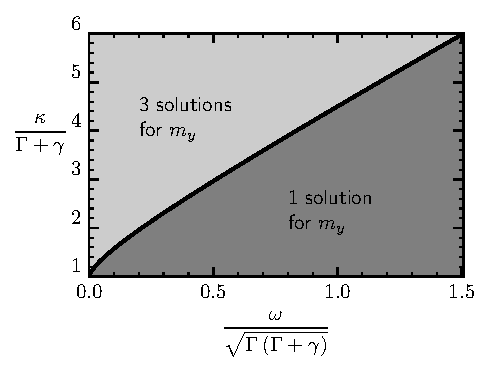
\includegraphics{pictures/numb_fixp.pdf}
    \vspace*{-2cm}\caption{The number of fixed points depending on the parameter configuration.}
    \label{fig:numb_fixp}
\end{wrapfigure}
With the rescaling $\Omega=\tw/\sqrt{2\,\Gamma\,(\Gamma+\gamma)}$ and $K=\tk/(\sqrt{2}\,(\Gamma+\gamma))$ we get
\begin{align*}
    B&=\frac{K}{2\,\Omega^2}
\end{align*}
and
\begin{align*}
    y_\text{max}&=\frac{1}{3}\,\left( 2+ \sqrt{1-\frac{3}{2}\,(1-K)\,\frac{1}{\Omega^2}}  \right)
\end{align*}
In this way we can compute the border between the configurations with different numbers of fixed points numerically. This is done by calculating the root of $F(y_{12})$ with respect to $K$ for various values of $\Omega$. As we know from previous considerations if $y_\text{max}<1$, i.e. $\tilde{A}>0$ which corresponds to $K>1$ the maximum of $F$ is negative even for $B=0$, resulting in only one solution. Another thing can be noted at this point. As $F(0)=-B$ and $B\neq0$ for $\kappa\neq0$, one solution $m_y$ has always to be negative for $\kappa\neq0$.\\\\
The next step in the examination is the analysis of the stability of the fixed points.
% \begin{figure}[H]
%     \hspace*{-1cm}
%     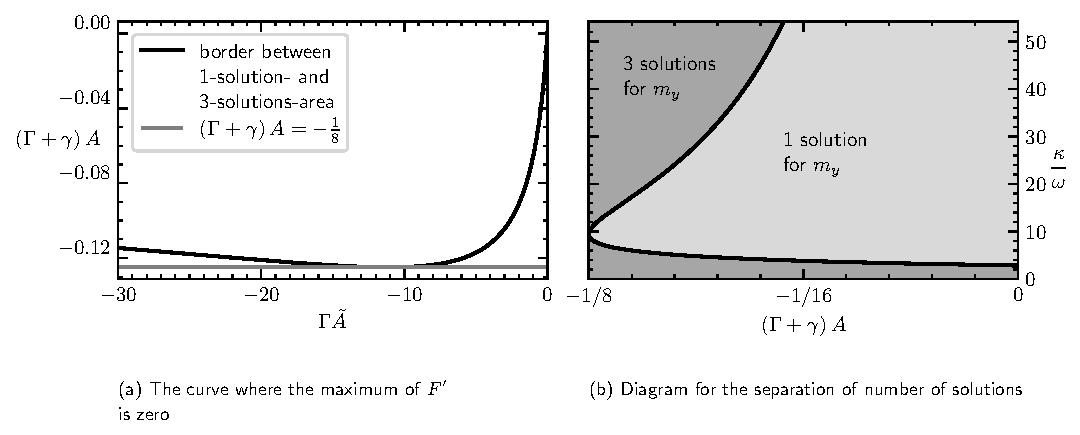
\includegraphics{pictures/phaseplot_A_kw.pdf}
%     \caption{The parameter configurations, where there are 1 ore 3 fixed points can be separated.}
%     \label{fig:phases_numb_of_fixp}
% \end{figure}
For this I proceed by calculating the linear expansion of the differential equations.
\begin{align*}
    \dt\left(\begin{array}{c}
         \delta m_x\\
         \delta m_y\\
         \delta m_z
    \end{array}\right)&=\left( \begin{array}{ccc}
        -\Gamma\,A-y^2+\frac{\tilde{\omega}}{\tilde{\kappa}}\,y&  0 & 0\\
        0 & -\Gamma\,A-y^2+\frac{\tilde{\omega}}{\tilde{\kappa}}\,y & \sqrt{2}\,\frac{\Gamma}{\tilde{\kappa}^2}\,(\tilde{\kappa}\,y-\tilde{\omega})\\
        0 &  -\sqrt{2}\,\frac{\Gamma}{\tilde{\kappa}^2}\,(2\tilde{\kappa}\,y-\tilde{\omega}) & -2\,\frac{\Gamma^2}{\tilde{\kappa}^2}
    \end{array} \right)\,\left(\begin{array}{c}
         \delta m_x\\
         \delta m_y\\
         \delta m_z
    \end{array}\right)
\end{align*}
For the analysis of the sign of the eigenvalues one is free to multiply the matrix with a positiv number, i.e $\tilde{\kappa}^2/\tilde{\omega}^2$, what yields the matrix
\begin{align*}
    \mathcal{A}=\left( \begin{array}{ccc}
        -\Gamma A-{y}^2+{y}&  0 & 0\\
        0 & -\Gamma A-{y}^2+{y}& \sqrt{2}\,\Gamma/\tilde{\kappa}\,({y}-\frac{\tilde{\kappa}}{\tilde{\omega}})\\
        0 &  -\sqrt{2}\,\Gamma/\tilde{\kappa}\,(2\,{y}-\frac{\tilde{\kappa}}{\tilde{\omega}}) & -2\,\frac{\Gamma^2}{\tilde{\omega}^2}
    \end{array} \right)
\end{align*}\newpage
The first eigenvalue is already accessible due to the block form of the matrix.
\begin{wrapfigure}[18]{l}{0pt}
    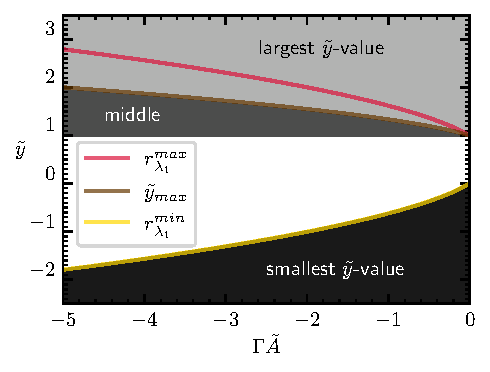
\includegraphics{pictures/sign_of_ev1.pdf}
    \vspace*{-2cm}\caption{The smaller ($r_{\lambda_1}^{min}$) and larger ($r_{\lambda_1}^{max}$) roots of $\lambda_1$ with marked areas for the value for ${y}=k/w\cdot m_y$. ${y}_{max}$ is the ${y}$-position of $F$.}
    \label{fig:sign_lam1}
\end{wrapfigure}\\
In order to allow oneself the answering of the question about the sign of the first eigenvalue in general, there can be defined an even more general parameter
\begin{align*}
    \chi\vcentcolon&=\frac{K-1}{\Omega^2}\\
    \Rightarrow\quad\Gamma A&=-\half\,\chi\\
    \frac{K}{2\,\Omega^2}&=\frac{K-1}{2\,\Omega^2}+\frac{1}{2\,\Omega^2}=\half\,\chi+\frac{1}{2\,\Omega^2}
\end{align*}
For a given value of $\chi$ the parameter $\Omega$ can be chosen freely, because through an appropriate choice of $K$ the value of $\chi$ can be fixed. So for every possible value of $\chi>0$ the supreme value of $B$ is just $\chi/2$, as $\Omega\rightarrow\infty$.

The first, smallest fixed point has again because of the positive sign of $B$ always a negative $y$-component. It has it's greatest value for minimal $B$. Negative values of $\chi$ lead to positive roots of $\lambda_1$, which induces that $\lambda_1$ itself is negative. \\\\
So one only has to consider positive $\chi$-values, in remembrance of fact, that there is only one fixed point for $\chi<0$ . It turns out that the smaller root of $\lambda_1$ is always a root of $F$ for $B=\chi/2$ and is therefore greater or equal the smallest root of $F$, and equal only for the border case, where $B=\chi/2$, what is of no interest.
\begin{align*}
    F({y})=-\half\,\chi-(1-\half\,\chi)\,{y}    - {y}^3+2\,{y}^2
\end{align*}
So we can move on to the next fixed point, the one in the middle. It takes it's smallest value for minimal $B$. In this constellation the middle root turns out to be always at ${y}=1$. The maximal possible value (actually supremum) for the middle root is at the maximum point of $F$ which is also the minimal possible value of the largest root. So we can already provide a diagramm for the possible sign-values of $\lambda_1$ in \autoref{fig:sign_lam1}.\\\\
At this point I want to discuss which of the above computed fixed points are physical ones, meaning $|m|<=1/2$. Therefore we consider the total mean angular momentum.
\begin{align*}
    m_z&=\half-\frac{1}{\Gamma}\,\left( \kappa\,(m_x^2+m_y^2)-\omega m_y  \right)\\
    &=\half-\frac{\kappa}{\Gamma}\,\left( m_y^2-\frac{\omega}{\kappa}\, m_y  \right)\\
    \Rightarrow\quad |m|^2&=\left( \half-\frac{\kappa}{\Gamma}\,\left( m_y^2-\frac{\omega}{\kappa}\, m_y  \right) \right)^2+m_y^2\\
    &=\left( \half-\frac{\omega^2}{\Gamma\kappa}\,\left( {y}^2- {y} \right) \right)^2+\frac{\omega^2}{\kappa^2}\,{y}^2\\
    &=\left( \half-\frac{\Omega^2}{K}\,\left( {y}^2- {y} \right) \right)^2+\frac{\Gamma}{\Gamma+\gamma}\,\frac{\Omega^2}{K^2}\,{y}^2\\
    \leq&\left( \half-\frac{\Omega^2}{K}\,\left( {y}^2- {y} \right) \right)^2+\frac{\Omega^2}{K^2}\,{y}^2\\
    &=\vcentcolon m^*
\end{align*}

Now I set $\Omega^2/K$ through the determining equation for $m_y$.
\begin{align*}
    0&=-\frac{K}{2\Omega^2}-\left( \frac{1-K}{2\Omega^2} +1\right)\,{y}-{y}^2+2\,{y}^2\\
    \Rightarrow\quad \frac{K}{2\Omega^2}\,({y}-1)&=(1+\frac{1}{2\Omega^2})\,{y}+{y}^3-2\,{y}^2\\
    \frac{\Omega^2}{K}&=\frac{{y}-1}{2\,\left(  (1+\frac{1}{2\Omega^2})\,{y}+{y}^3-2\,{y}^2\right)}
\end{align*}
\begin{align*}
    \frac{\text{d}}{\text{d}{y}}\,\frac{\Omega^2}{K}&=\frac{1}{2\,\left(  (1+\frac{1}{2\Omega^2})\,{y}+{y}^3-2\,{y}^2\right)}-\frac{2\,({y}-1)\,(1+\frac{1}{2\Omega^2}+3\,{y}^2-4\,{y})}{4\,\left(  (1+\frac{1}{2\Omega^2})\,{y}+{y}^3-2\,{y}^2\right)^2}\\\\
    &=\frac{1+\frac{1}{2\Omega^2}-4\,{y}+5\,{y}^2-2\,{y}^3}{2\,\left(  (1+\frac{1}{2\Omega^2})\,{y}+{y}^3-2\,{y}^2\right)^2}
\end{align*}

This equation looks at first strange, because $k/2\Omega^2$ could be negative for $0<{y}<1$. But as we've already seen in \autoref{fig:sign_lam1}, this space is free of fixed points. \\\\
Taking the derivative of $m^*$
\begin{align*}
    \frac{\partial m^*}{\partial{y}}&=-2\,\left(\frac{\Omega^2}{K}\,(2{y}-1)+\left(\frac{\text{d}}{\text{d}{y}}\,\frac{\Omega^2}{K}\right)\,({y}^2-{y})\right)\,\left( \half-\frac{\Omega^2}{K}\,\left( {y}^2- {y} \right) \right)+2\,\frac{\Omega^2}{K^2}\,{y}+2\,\left(\frac{\text{d}}{\text{d}{y}}\,\frac{\Omega^2}{K}\right)\,\frac{\Omega^2}{K}\,\frac{1}{\Omega^2}\,{y}^2\\\\
    &=4\,(\frac{\Omega^2}{K})^2\,{y}^3-\left(2\,(\frac{\Omega^2}{K})^2+4\,(\frac{\Omega^2}{K})^2\right)\,{y}^2+\left( 2\,(\frac{\Omega^2}{K})^2+2\,\frac{\Omega^2}{K^2}-2\,\frac{\Omega^2}{K} \right)\,{y}+\frac{\Omega^2}{K}\\\\
    &+2\,\dkw\,\kw\,{y}^4-4\,\dkw\,\kw\,{y}^3\\\\
    &-\left(\dkw-2\,\dkw\,\kw-2\,\dkw\,\kw\,\frac{1}{\Omega^2}\right)\,{y}^2+\dkw\,{y}\\\\
    &=\frac{\Omega^2}{K}\,\left[  4\,\frac{\Omega^2}{K}\,{y}^3-6\,\frac{\Omega^2}{K}\,{y}^2+\left( 2\,\frac{\Omega^2}{K}+2\,\frac{\Omega^2}{K}\,\frac{1}{\Omega^2}-2 \right)\,{y}+1 \right]\\\\
    &+\dkw\,\left[2\,\kw\,{y}^4-4\,\kw\,{y}^3-\left(1-2\,\kw-2\,\kw\,\frac{1}{\Omega^2}\right)\,{y}^2+{y}\right]\\\\
    &=\vcentcolon \frac{\partial \alpha}{\partial{y}}+\dkw\,\frac{\partial \beta}{\partial{y}}
\end{align*}

So plugging the found result into the equation for the derivative of $m^*$ yields
\begin{align*}
    \frac{2\,\left[(1+\frac{1}{2\Omega^2})\,{y}+{y}^3-2\,{y}^2\right]^2}{{y}-1}\,\frac{\partial \alpha}{\partial{y}}&=2\,({y}-1)\,{y}^3-3\,({y}-1)\,{y}^2\\
    &+\left( {y}-1+({y}-1)\,\frac{1}{\Omega^2}-2\,\left((1+\frac{1}{2\Omega^2})\,{y}+{y}^3-2\,{y}^2\right) \right)\,{y}\\
    &+(1+\frac{1}{2\Omega^2})\,{y}+{y}^3-2\,{y}^2 \\\\
    &=3\,{y}^2+\left( -(1+\frac{1}{\Omega^2})-{y}\right)\,{y}+(1+\frac{1}{2\Omega^2})\,{y}-2\,{y}^2\\
    &=-\frac{1}{2\Omega^2}\,{y}\\\\
    \Rightarrow\quad\frac{\partial \alpha}{\partial{y}}&=-\frac{{y}-1}{2\,\left[(1+\frac{1}{2\Omega^2})\,{y}+{y}^3-2\,{y}^2\right]^2}\,\frac{1}{2\Omega^2}\,{y}
\end{align*}
Doing the same for the $\beta$-expression
\begin{align*}
    \left[(1+\frac{1}{2\Omega^2})\,{y}+{y}^3-2\,{y}^2\right]\,\frac{\partial \beta}{\partial{y}}&=({y}-1)\,{y}^4-2\,({y}-1)\,{y}^3-\left( (1+\frac{1}{2\Omega^2})\,{y}+{y}^3-2\,{y}^2-{y}+1-({y}-1)\,\frac{1}{\Omega^2} \right)\,{y}^2\\
    &+((1+\frac{1}{2\Omega^2})\,{y}+{y}^3-2\,{y}^2)\,{y}\\
    &=-\left( 1+\frac{1}{\Omega^2}-\frac{1}{2\Omega^2}\,{y}  \right)\,{y}^2+(1+\frac{1}{2\Omega^2})\,{y}^2\\
    &=\frac{1}{2\Omega^2}\,({y}^3-{y}^2)=\frac{1}{2\Omega^2}\,{y}^2\,({y}-1)
\end{align*}
Collecting the terms together, it is found
\begin{align*}
    \frac{\partial \alpha}{\partial{y}}+\dkw\,\frac{\partial \beta}{\partial{y}}&=-\frac{\frac{1}{2\Omega^2}\,({y}-1)}{2\,\left[(1+\frac{1}{2\Omega^2})\,{y}+{y}^3-2\,{y}^2\right]^3}\,\left( {y}\,((1+\frac{1}{2\Omega^2})\,{y}+{y}^3-2\,{y}^2) -{y}^2\,(1+\frac{1}{2\Omega^2}-4\,{y}+5\,{y}^2-2\,{y}^3)\right)\\
    &=-\frac{\frac{1}{2\Omega^2}\,({y}-1)}{2\,\left[(1+\frac{1}{2\Omega^2})\,{y}+{y}^3-2\,{y}^2\right]^3}\,\left( 2\,{y}^5-4\,{y}^4+2\,{y}^3 \right)\\
    &=-\frac{\frac{1}{2\Omega^2}\,({y}-1)}{2\,\left[(1+\frac{1}{2\Omega^2})+{y}^2-2\,{y}\right]^3}\,\left( 2\,{y}^2-4\,{y}+2 \right)
\end{align*}
We can examine the roots of the two quadratic polynomials in numerator and denominater
\begin{align*}
    2\,{y}^2-4\,{y}+2\rightarrow\text{roots}&=\frac{1}{4}\,(4\pm\sqrt{16-16})\\
    &=1\\
    \Rightarrow\quad 2\,{y}^2-4\,{y}+2&=2\,({y}-1)^2\\
    (1+\frac{1}{2\Omega^2})+{y}^2-2\,{y}\rightarrow\text{roots}&=\half\,(2\pm\sqrt{4-4\,(1+\,\frac{1}{2\Omega^2})})\\
    &=2\pm\sqrt{-\frac{1}{2\Omega^2}}
\end{align*}
So the denominator is always larger then zero
\begin{align*}
    \frac{\partial m^*}{\partial{y}}&=-\frac{\frac{1}{2\Omega^2}\,({y}-1)^3}{\left[(1+\frac{1}{2\Omega^2})+{y}^2-2\,{y}\right]^3}
\end{align*}
We see here that $\partial_{{y}}\,m^*>0$ for ${y}<1$ and $\partial_{{y}}\,m^*<0$ for ${y}>1$. So for the two areas in which ${y}$ can fall, for the one smaller than zero $m^*$ takes it's maximum for ${y}\rightarrow0$ and for the area ${y}>1$ $m^*$ takes it's maximum for ${y}\rightarrow1$. Looking again of the form of $|m|^2$ 
\begin{align*}
    |m|^2\leq m^*\left( \half-\frac{\Omega^2}{K}\,\left( {y}^2- {y} \right) \right)^2+\frac{\Omega^2}{K^2}\,{y}^2
\end{align*}
we can say $m^*({y}\rightarrow0)=1/4$. The limit of ${y}\rightarrow1$ can only be achieved in the limit $\Omega\rightarrow\infty$, while% i.e. $\Gamma/\omega^2\rightarrow0$, while
\begin{align*}
    \text{constant}=\frac{K}{\Omega^2}=\frac{\kappa\Gamma}{\omega^2}
\end{align*}
This means in particular, that also $K\rightarrow\infty$ and therefore $K^2/\Omega^2\rightarrow\infty$. But this fixes $|m|$ to $1/2$. 
\begin{figure}[H]
    \hspace*{-1cm}
    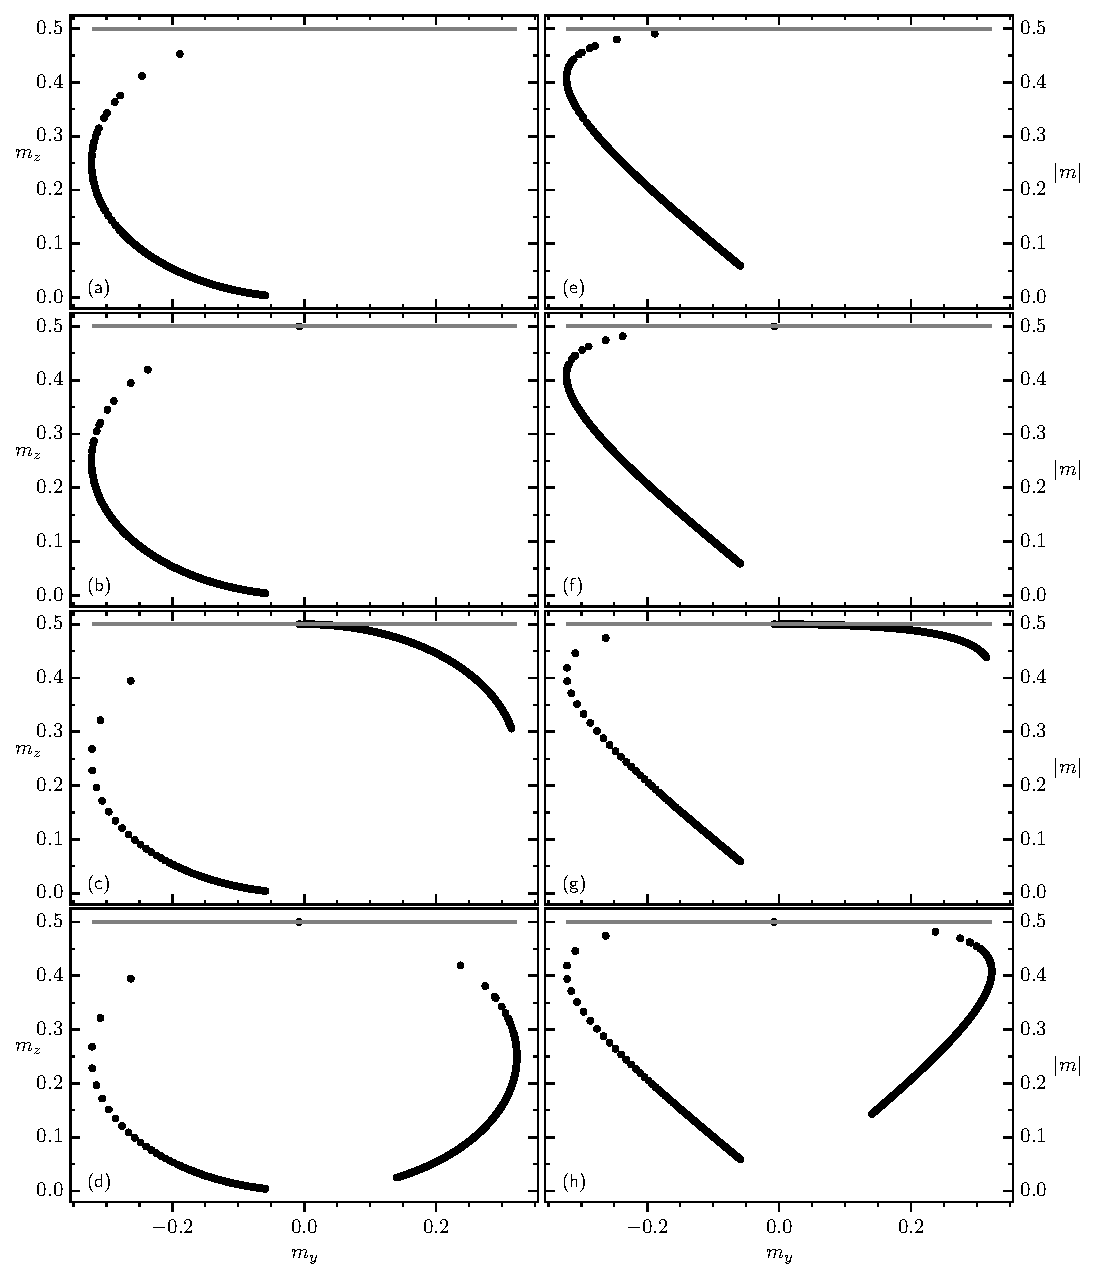
\includegraphics{pictures/fixp_boundaries.pdf}
    \caption{This graphic showes the range of $m_y$, $m_z$, $|m|$ for a parameter grid of $1.2\leq\kappa\leq24$ and $3\cdot10^{-7}\leq\omega\leq7$, $\Gamma=1$ $\gamma=0.2$. In the left column (a-d) the fixed points are shown in the $y-z$-plane, whereas in the right column (e-h) the modulus of the total angular momentum is depectid in dependence of $m_y$ for the different parameter values. The first row shows the fixed point in the parameter regime, where there is only one fixed point. From the 2. row downwards the fixed points in the area of three stationary solutions are show in the order smallest, middle and largest $m_y$-value.}
\end{figure}

\begin{figure}[H]
    \hspace*{-1cm}
    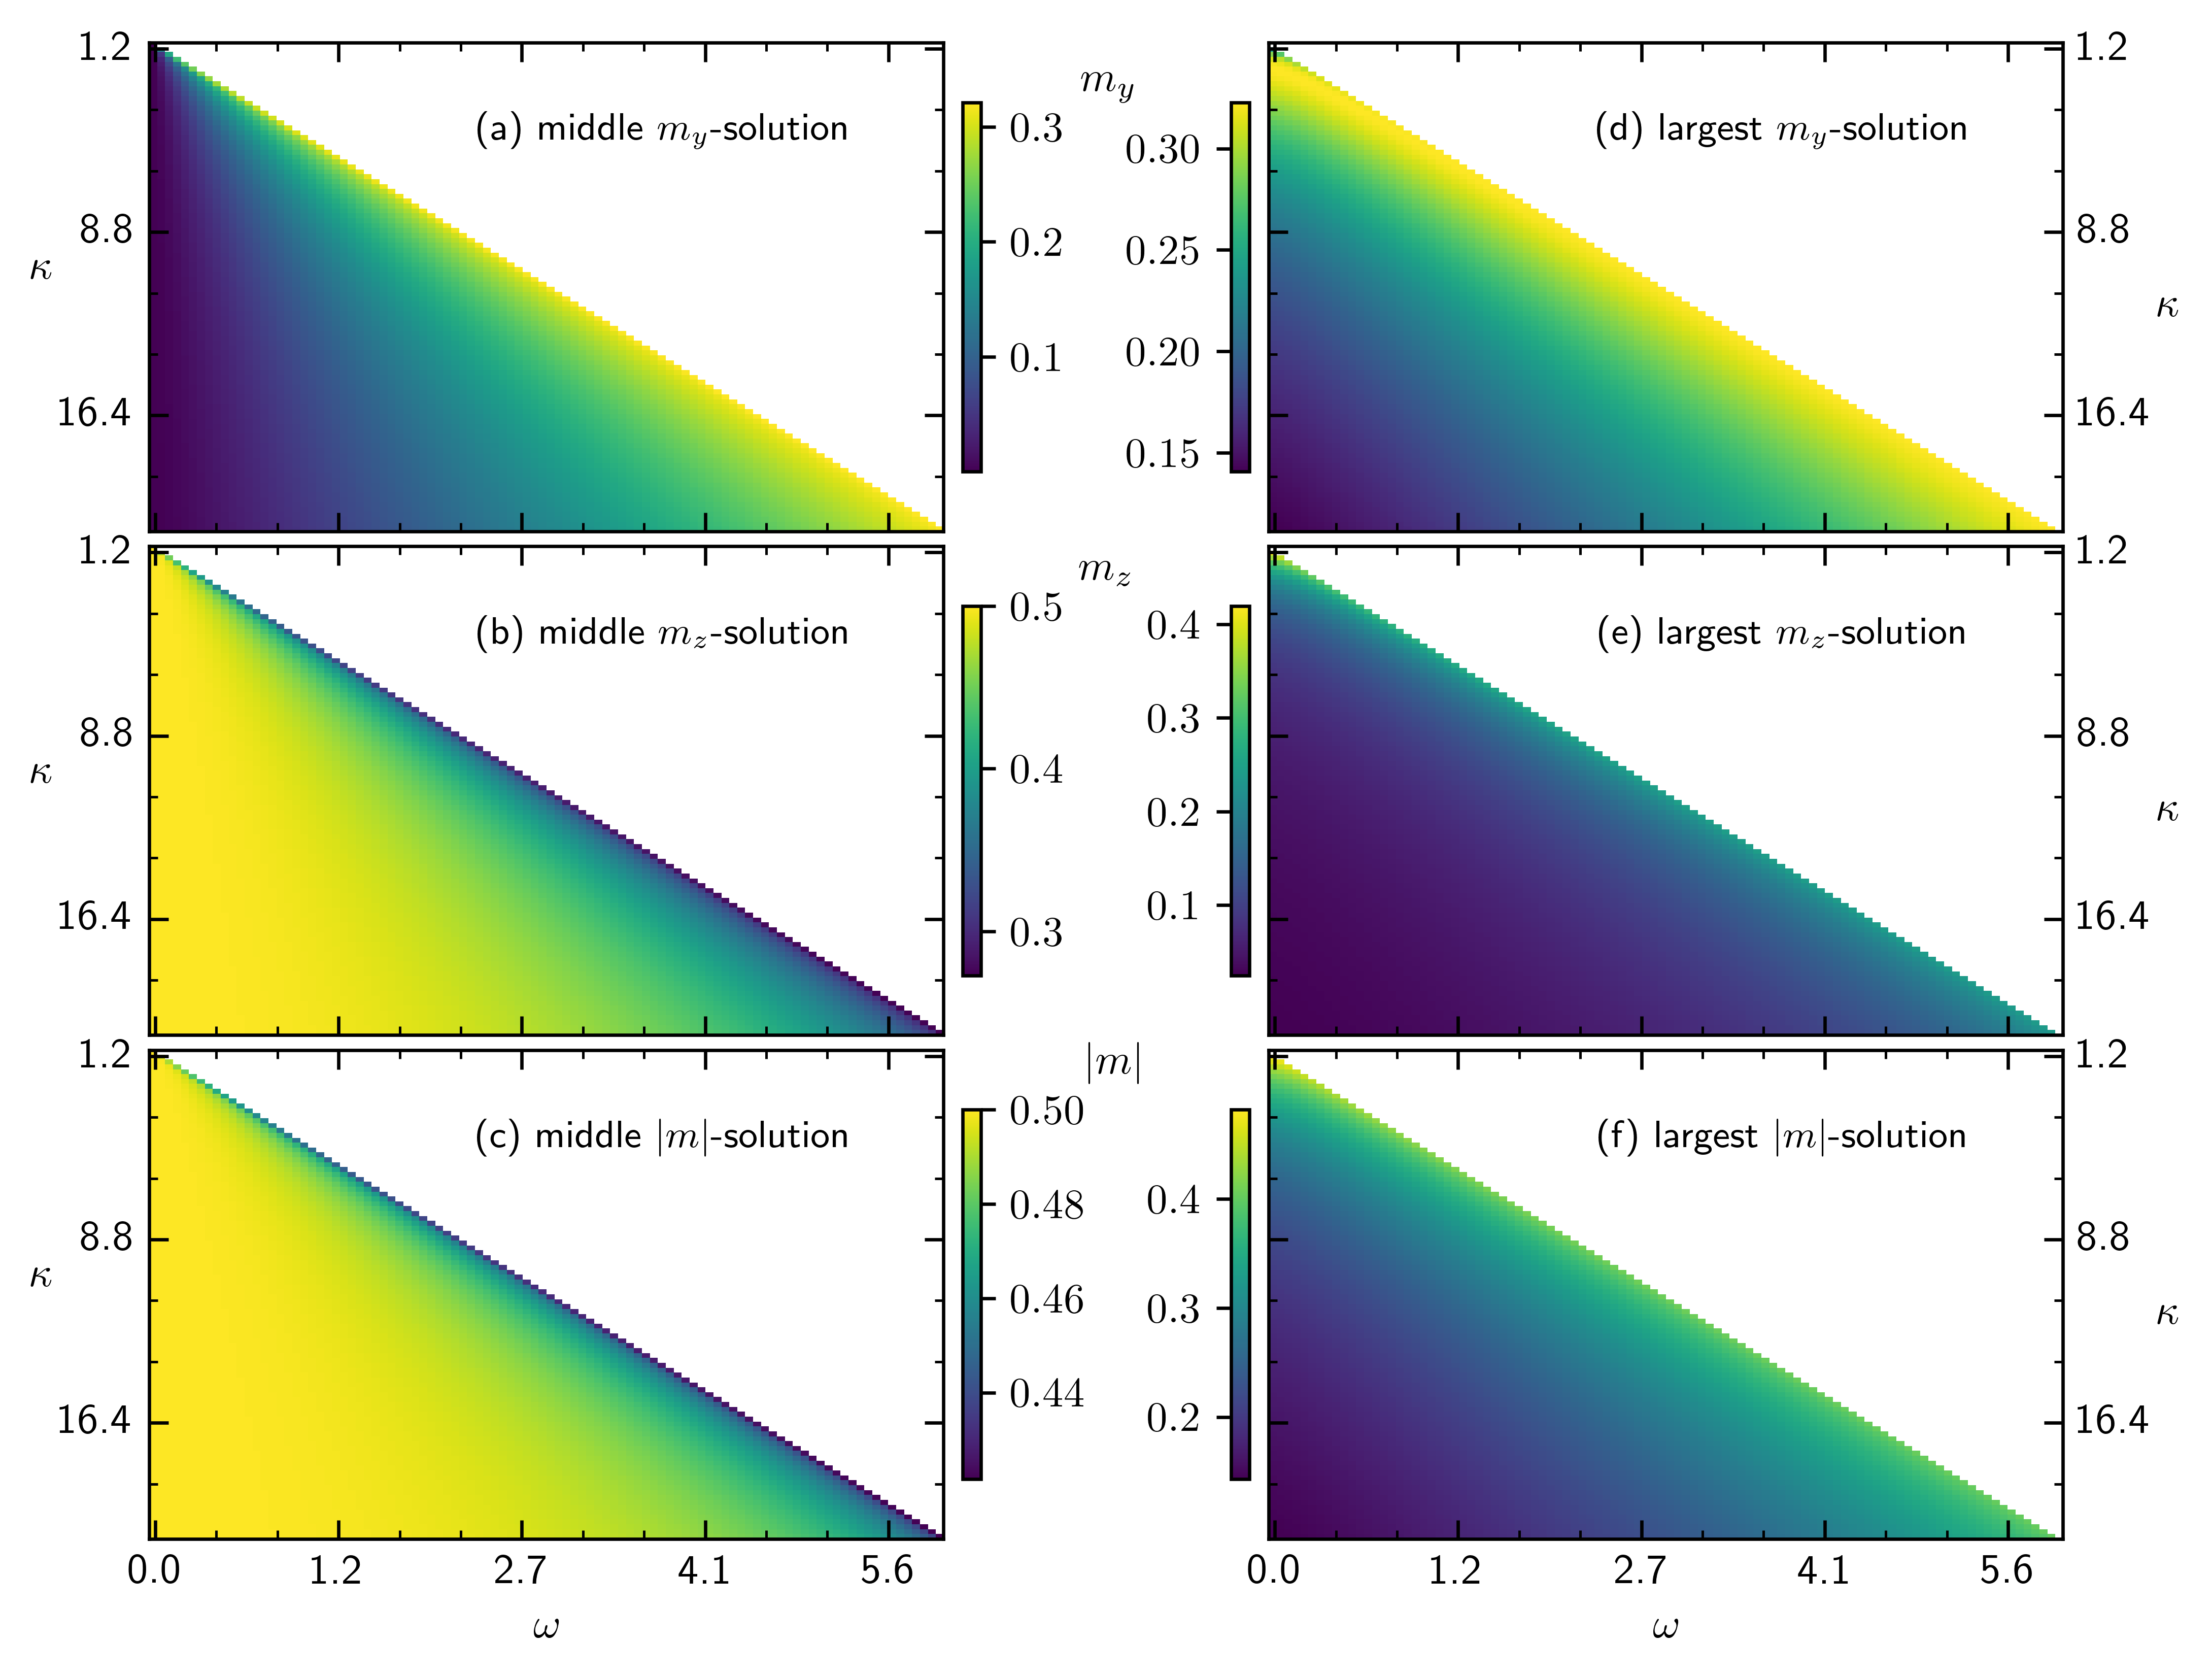
\includegraphics{pictures/fixp_bound_heatmap_ml.png}
    \caption{heatmap of the range of the fixed point for a certain parameter range of $\omega$ and $\kappa$. $\Gamma=1$, $\gamma=0.2$ are fixed. Shown are the middle and larger $m_y$-solutions.}
    \label{fig:fixp_midlarge_bound_hm}
\end{figure}




\begin{appendices}

\section{Derivation of the equations of motion}
\label{appendix:eqm_derv}

For the calculations with Pauli matrices revise a few of their properties.
\begin{align*}
    [\sigma^\alpha,\sigma^\beta]&=2i\,\varepsilon_{\alpha\beta\lambda}\,\sigma^\lambda\\
    \Rightarrow\quad[J_\alpha,J_\beta]&=i\,\varepsilon_{\alpha\beta\lambda}\,J_\lambda\\
    [\sigma^z,\sigma^\pm]&=\pm2\,\sigma^\pm\\
    \Rightarrow\quad[J_z,J_\pm]&=\pm J_\pm\\
    \sigma^x\sigma^z&=\left( \begin{array}{cc}
         0 & -1  \\
         1& 0
    \end{array}\right)=-i\,\sigma^y\\
    \sigma^y\sigma^z&=\left( \begin{array}{cc}
         0 & i  \\
         i& 0
    \end{array}\right)=i\,\sigma_x\\
    \sigma^x\sigma^y&=\left( \begin{array}{cc}
         i & 0  \\
         0 & -i
    \end{array}\right)=i\,\sigma_z\\
    \sigma^\pm\sigma^z&=-i\,\sigma^y\pm i^2\,\sigma^x=\mp\sigma^\pm\\
    \sigma^-\sigma^+&=(\sigma^x)^2+(\sigma^y)^2+i\,\sigma^x\sigma^y-i\,\sigma^y\sigma^x\\
    &=2-2\,\sigma^z\\
    \sigma^+\sigma^-&=(\sigma^x)^2+(\sigma^y)^2-i\,\sigma^x\sigma^y+i\,\sigma^y\sigma^x\\
    &=2+2\,\sigma^z\\
    [\sigma^+,\sigma^-]_-&=4\,\sigma^z
\end{align*}
From this the different contributions to the Lindblad follow.
\begin{align*}
    \mathcal{L}_S(J_z)&=-i\,\omega\,\braket{[J_z,J_x]}\\
    &=\omega\,\braket{J_y}\\
    \mathcal{L}_S(J_\pm)&=-i\,\frac{\delta}{2}\,\braket{[J_\pm,J_z]}-i\,\omega\,\braket{[J_\pm,J_x]}\\
    &=-i\,\left(\mp\frac{\delta}{2}\, \braket{J_\pm} \pm \omega\, \braket{J_z}\right)
\end{align*}

\begin{align*}
    \mathcal{L}_a(J_z)&=\frac{\kappa}{N}\,\Trs{\left(J_+ J_z J_- \rho-\half\,[J_z,J_+ J_-]_+\,\rho\right)}\\
    &=\frac{\kappa}{N}\,\Trs{\left(J_z J_+ J_- - J_+ J_- -\half\,(J_z J_+ J_- + J_+ J_z J_- + J_+ J_-)\right)\,\rho}\\
    &=\frac{\kappa}{N}\,\Trs{\left(J_z J_+ J_- - J_+ J_- -\half\,(2\,J_z J_+ J_- + J_+ J_- - J_+ J_-)\right)\,\rho}\\
    &=-\frac{\kappa}{N}\,\Trs{J_+ J_- \rho}\\\\
    \mathcal{L}_a(J_+)&=\frac{\kappa}{N}\,\Trs{\left(J_+ J_+ J_- \rho-\half\,[J_+,J_+ J_-]_+\,\rho\right)}\\
    &=\frac{\kappa}{N}\,\Trs{\left(J_+ J_- J_+ + 2\,J_+ J_z -\half\,(J_+ J_- J_+ + J_+ J_+ J_-)\right)\,\rho}\\ &=\frac{\kappa}{N}\,\Trs{\left(J_+ J_- J_+ + 2\,J_+ J_z -\half\,(2\,J_+ J_- J_+ + 2 J_+ J_z)\right)\,\rho}\\\\
    &=\frac{\kappa}{N}\,\Trs{J_+ J_z \rho}\\\\
    \mathcal{L}_a(J_-)&=\frac{\kappa}{N}\,\Trs{\left(J_+ J_- J_- \rho-\half\,[J_-,J_+ J_-]_+\,\rho\right)}\\
    &=\frac{\kappa}{N}\,\Trs{\left(J_- J_+ J_- + 2\,J_z J_- -\half\,(J_- J_+ J_- + J_+ J_- J_-)\right)\,\rho}\\ 
    &=\frac{\kappa}{N}\,\Trs{J_z J_- \rho}
\end{align*}
\begin{align*}
    \mathcal{L}_b(J_z)&=0\\
    \mathcal{L}_b(J_\pm)&=\gamma\,\Trs{\left(J_z J_\pm J_z \rho-\half\,[J_\pm,J_z^2]_+\,\rho\right)}\\
    &=\gamma\,\Trs{\left(J_\pm J_z^2\rho \pm J_\pm J_z \rho-\half\,(J_\pm J_z^2 + J_z J_\pm J_z \pm J_z J_\pm)\,\rho\right)}\\
    &=\gamma\,\Trs{\left(J_\pm J_z^2\rho \pm J_\pm J_z \rho-\half\,(2\,J_\pm J_z^2  \pm J_z J_\pm \pm J_\pm J_z)\,\rho\right)}\\
    &=\pm\half\, \gamma\,\Trs{[J_\pm,J_z]\,\rho}\\
    &=-\half\,\gamma\,\Trs{J_\pm\rho}
\end{align*}
\begin{align*}
    \mathcal{L}_c(J_z)&=\frac{\Gamma}{8}\,\sum_{j,k=1}^N \Trs{\left( \sigma_j^- \sigma_k^z \sigma_j^+ -\half\,[\sigma_k^z,\sigma_j^-\sigma_j^+]_+   \right)\,\rho}\\
    &=\frac{\Gamma}{8}\,\sum_{j,k=1}^N \Trs{\left( \sigma_j^- \sigma_k^z \sigma_j^+ -\half\,[\sigma_k^z\sigma_j^-\sigma_j^++\sigma_j^-\sigma_j^+\sigma_k^z]   \right)\,\rho}\\
    &=\frac{\Gamma}{8}\,\sum_{j,k=1}^N \Trs{\left( \sigma_j^- \sigma_k^z \sigma_j^+ -\half\,[2\,\sigma_j^-\sigma_k^z\sigma_j^+  -2\, \sigma_j^-\sigma_j^+\delta_{jk}-2\, \sigma_j^-\sigma_j^+\delta_{jk}]   \right)\,\rho}\\
    &=\frac{\Gamma}{8}\,\sum_{k=1}^N \Trs{2\, \sigma_k^-\sigma_k^+  \,\rho}\\
    &=\frac{\Gamma}{4}\,\sum_{k=1}^N \Trs{ (2-2\,\sigma_k^z)  \,\rho}\\
    &=\half\,N\,\Gamma-\Gamma\,\braket{J_z}
\end{align*}
\begin{align*}
    \mathcal{L}_c(J_-)&=\frac{\Gamma}{4}\,\sum_{j,k=1}^N \Trs{\left( \sigma_j^- \sigma_k^- \sigma_j^+ -\half\,[\sigma_k^-,\sigma_j^-\sigma_j^+]_+   \right)\,\rho}\\
    &=\frac{\Gamma}{4}\,\sum_{k=1}^N \Trs{\left( \sigma_k^- \sigma_k^- \sigma_k^+ -\half\,[\sigma_k^-\sigma_k^-\sigma_k^++\sigma_k^-\sigma_k^+\sigma_k^-]   \right)\,\rho}\\
    &=-\frac{\Gamma}{2}\,\sum_{k=1}^N\Trs{\sigma_k^-\sigma_k^z\rho}\\
    &=-\frac{\Gamma}{2}\,\sum_{k=1}^N\Trs{\sigma_k^-\rho}\\\\
    \mathcal{L}_c(J_+)&=\frac{\Gamma}{4}\,\sum_{j,k=1}^N \Trs{\left( \sigma_j^- \sigma_k^+ \sigma_j^+ -\half\,[\sigma_k^+,\sigma_j^-\sigma_j^+]_+   \right)\,\rho}\\
    &=-\frac{\Gamma}{2}\,\sum_{k=1}^N\Trs{\sigma_k^z\sigma_k^+\rho}\\
    &=-\frac{\Gamma}{2}\,\sum_{k=1}^N\Trs{\sigma_k^+\rho}
\end{align*}

\section{The J-square calculus}
\label{appendix:msq_calc}
If there is a system of $N$ coupled ODE, this could be seen as the quest for a function $\vec{F}:\,\mathbb{R}\rightarrow\mathbb{R}^N$. Derived from that, there can also be defined the function squared $F^2:\,\mathbb{R}\rightarrow\mathbb{R}:\,t\mapsto\sum_{i=1}^NF_i^2(t)$. If one is now able to write the derivative of squared function in the following way
\begin{align*}
    \dt F^2(t)&=\vec{F}^t(t)\,A\,\vec{F}(t)
\end{align*}
with a Matrix $A$, which is positive ore negative definite, then there do not exist stationary solutions to the system of ODE, including limit cycles. \\
\textit{Proof}: The functions $\vec{F}$, can be mapped via N-dimensional spherical coordinates into a different set of functions $f(t)$, $\varphi_j(t)$ $j\in\{1,\dots,N-1\}$, with $f$ the modulus of $F$, and $\varphi_j$ the angles. This is true for all solutions $\vec{F}\neq\vec{0}$. In the following we neglect this special case, as this is in the most cases anyway a stationary point. With the notation.
\begin{align*}
    \vec{F}(t)&=f(t)\,\hat{r}(t)
\end{align*}
we can rewrite the differential equation for the squared function to
\begin{align*}
    \dt F^2(t)=\dt f^2(t)=2\,f(t)\,\dt f(t)&=f^2(t)\,\hat{r}^t\,A\,\hat{r}\\
    \Rightarrow\quad\dt f(t) = f(t)\,\hat{r}^t\,A\,\hat{r}
\end{align*}
Assuming that A is positive or negative definite we can use the property that $|\hat{r}(t)|=1\,\forall t$, in order to follow, that there exists an $\varepsilon>0$ so that
\begin{align*}
    \lambda(t)\vcentcolon=\left| \hat{r}^t(t)\,A\,\hat{r}(t) \right| > \varepsilon
\end{align*}
For all $t$ and all functions $\{\varphi_j(t)\}$. \textit{Proof}: if this doesn't hold, there will have to be a sequence $(t_n)$ with $\lambda(t_n)\rightarrow0$. As the surface of an N-dimensional sphere is a compact set, this sequence would have to converge on the survace of the sphere, which would infer $\exists \hat{r}\neq0$ with 
\begin{align*}
    \hat{r}^t(t)\,A\,\hat{r}(t)=0
\end{align*}
in contradiction to the definiteness of $A$. So depending on, whether $A$ is positive or negative definite, we can write
\begin{align*}
    \dt f(t) >& \varepsilon\,f(t)\\
    \Rightarrow\quad f(t) >& c\,e^{\varepsilon\,t}\\
    \text{or}\quad \dt f(t) <& -\varepsilon\,f(t)\\
    \Rightarrow\quad f(t) <& c\,e^{-\varepsilon\,t}\\
\end{align*}
for suitable choice of $c$ (can be shown with mean value theorem). This implies, that there can't be a stationary solution of the set of ODE. The last statement holds, because for $t\rightarrow\infty$ either $f$ goes to zero, which would imply that all $F_i$ go to zero or $f$ grows boundlessly, which implies that, independent of the starting conditions, there exists a $F_i$, that grows boundlessly, which forbids the properties of a stationary state including limit cycles.



\end{appendices}

\printbibliography

\end{document}
% Both can be implemented through stationary electric and magnetic fields, which are described in a semi-classical way. The possibility to treat the field classically arises, when the fields are very off resonant to the atomic transition considered. This is certainly the case if the field is assumed to be static. In this case the Zeeman and Stark effect come into play, which are described through a classical field.